\documentclass[11pt,a4paper]{article}

% ---------- Packages ----------
\usepackage[margin=0.85in]{geometry}
\usepackage[T1]{fontenc}
\usepackage[utf8]{inputenc}
\usepackage{lmodern}
\usepackage[protrusion=true,expansion=false]{microtype}
\usepackage{graphicx}
\usepackage{subcaption}
\usepackage{booktabs}
\usepackage{amsmath,amssymb}
\usepackage{xcolor}
\usepackage[hidelinks]{hyperref}
\usepackage{titlesec}
\usepackage{caption}
\usepackage{enumitem}

% ---------- Layout tweaks ----------
\graphicspath{{../outputs/figures/}}
\captionsetup{font=small,labelfont=bf,skip=3pt}
\setlength{\parskip}{0.30em}
\setlength{\parindent}{0pt}
\setlist[itemize]{leftmargin=1.2em,itemsep=1pt,topsep=1pt}
\titlespacing*{\section}{0pt}{0.9ex}{0.3ex}
\titlespacing*{\subsection}{0pt}{0.6ex}{0.2ex}
\titleformat{\section}{\normalfont\Large\bfseries}{\thesection.}{0.5em}{}
\titleformat{\subsection}{\normalfont\large\bfseries}{\thesubsection}{0.5em}{}

% Accent color for title page
\definecolor{accent}{HTML}{1F3A5F}

\begin{document}

% =====================================================================
% TITLE PAGE (not counted toward 6-page limit)
% =====================================================================
\begin{titlepage}
\centering
\vspace*{1.4cm}

{\large\scshape National University of Singapore \\[0.2em] School of Computing \par}
\vspace{0.5cm}
{\large BT4014 Analytics Driven Design of Adaptive Systems \par}
{\normalsize Academic Year 2025/2026 --- Semester 2 \par}

\vspace{1.2cm}
{\color{accent}\rule{0.85\textwidth}{1.2pt}}
\vspace{0.3cm}

% Title block with thin vertical accents on left and right,
% horizontal rules above and below.
\noindent
\begin{minipage}{0.04\textwidth}
    \centering\color{accent}\rule[-3.7cm]{1.2pt}{4.2cm}
\end{minipage}\hfill
\begin{minipage}{0.88\textwidth}
    \centering
    \vspace{0.2cm}
    {\Huge\bfseries Adaptive Job-Application UI Selection \par}
    \vspace{0.35em}
    {\Huge\bfseries with Contextual Bandits \par}
    \vspace{0.8cm}
    {\large\itshape A large-scale simulated benchmark of contextual \\[0.1em]
    versus non-contextual bandit policies for \\[0.1em]
    adaptive job-search interface routing \par}
\end{minipage}\hfill
\begin{minipage}{0.04\textwidth}
    \centering\color{accent}\rule[-3.7cm]{1.2pt}{4.2cm}
\end{minipage}

\vspace{0.3cm}
{\color{accent}\rule{0.85\textwidth}{1.2pt}}

\vfill

{\Large\bfseries Group X \par}
\vspace{0.6cm}

{\large
\begin{tabular}{rl}
REDACTED             & \texttt{REDACTED} \\[0.15em]
REDACTED             & \texttt{REDACTED} \\[0.15em]
REDACTED             & \texttt{REDACTED} \\[0.15em]
REDACTED             & \texttt{REDACTED} \\
\end{tabular}
\par}

\vfill

{\color{accent}\rule{0.5\textwidth}{0.4pt}}\\[0.5em]
{\normalsize Final Project Report \par}
{\normalsize 24 April 2026 \par}
\vspace{0.5cm}

\end{titlepage}

% =====================================================================
% BODY --- 6 pages
% =====================================================================
\setcounter{page}{1}

% ---------------------------------------------------------------------
\section{Introduction}

Job-search platforms serve the same opportunities through very different
interfaces: a LinkedIn-style split pane, a Tinder-like swipe view, a dense card
grid, a chatbot-guided flow, or a hybrid ranked feed. Which interface produces
the most successful applications is not a single design choice but a
\emph{policy}: the best UI for a rushed ``panic apply'' session may be the worst
UI for a deliberate senior-level job search. We therefore pose the platform's
design problem as a contextual multi-armed bandit: at each round, the system
observes an applicant/job/company/session context, picks one of five UI arms,
and receives a scalar reward tied to first-round interview outcomes.

Because no public dataset logs applicant-level UI exposure and callback outcomes
jointly, we build a procedural simulator large enough for online regret
analysis ($1{,}050{,}000$ rounds per policy, $5{,}250{,}000$ algorithm-rounds
total) and calibrate it so different session goals favour different arms. We
then compare two context-aware policies (LinUCB, Contextual Thompson Sampling)
against three non-contextual baselines ($\varepsilon$-Greedy, UCB1, Gaussian
Thompson Sampling).

\textbf{Main finding.} Contextual methods reduce cumulative expected regret by
$43$--$47\%$ relative to the best non-contextual baseline. The advantage is
\emph{not} uniform: it is largest where the oracle-best arm differs sharply by
session goal, and almost vanishes in ``panic apply'' sessions where the
exploration overhead of contextual methods actually hurts. The learned-policy
heatmap (Figure~\ref{fig:learned-policy}) makes the mechanism explicit:
contextual methods route arms per session goal while non-contextual methods
collapse to a single globally strong interface.

% ---------------------------------------------------------------------
\section{Data and Context}

\subsection{Platform context and problem}

The target platform is an adaptive job-search service that chooses, for each
applicant session, which application interface (\emph{arm}) to serve. Five arms
match the dominant UI archetypes in the market: \texttt{panel\_split} (list +
detail pane), \texttt{card\_grid} (dense card scroll), \texttt{swipe\_fast}
(one-at-a-time accept/skip), \texttt{guided\_chat} (conversational narrowing),
and \texttt{hybrid\_ranked} (ranked shortlist with expandable detail). Each arm
differs in information density, reading cost, fatigue impact, and self-filtering
quality rather than in the underlying job pool. Because no production platform
has run such an adaptive policy, no historical dataset logs UI-specific
outcomes for counterfactual arms, which motivates a simulation-based study.

\subsection{Synthetic data generation}

The simulator is built in a layered, hierarchical fashion: global ontologies
$\rightarrow$ static entities $\rightarrow$ sessions $\rightarrow$ per-round
interactions. Entity scales and session-level intent distributions are fixed
up-front and do not depend on the bandit's behaviour.

\textbf{Entities (static).}
$200{,}000$ applicants are drawn from six cohorts (\texttt{new\_grad},
\texttt{junior\_generalist}, \texttt{mid\_specialist}, \texttt{senior\_specialist},
\texttt{career\_switcher}, \texttt{burned\_out\_mass\_applier}), each with a
$24$-dimensional skill vector and ten behavioural traits (reading patience,
decision speed, fatigue sensitivity, scatter-apply tendency, resume quality,
etc.). $8{,}000$ companies are partitioned into five tiers
(\texttt{small\_local}, \texttt{startup}, \texttt{mid\_market},
\texttt{large\_public}, \texttt{elite\_platform}), each carrying a \emph{static}
evaluation rubric: per-feature screening weights $w_c=(w_s, w_e, w_d, w_k,
w_c^{\mathrm{cl}},\ldots)$ summing to one, fixed
\texttt{ignore}/\texttt{interview} thresholds, and a company value weight
$w^{\mathrm{val}}_c\in[0.8,1.5]$. This static rubric is the ground-truth
environment; the bandit never modifies it. $120{,}000$ jobs are generated
conditional on company tier and role family. $300{,}000$ sessions are drawn
with four goal labels: \texttt{focused\_search}, \texttt{broad\_exploration},
\texttt{panic\_apply}, \texttt{casual\_browse}.

\textbf{Context vector.}
At each round $t$ the platform observes $x_t \in \mathbb{R}^{48}$ assembled
from an applicant block (12 dims), a job block (10), a company block (8), a
session block (8), and engineered cross-features (10, including
\texttt{skill\_match}, \texttt{keyword\_match}, \texttt{ui\_need}, and an
\texttt{applicant\_uncertainty} score).

\textbf{Reward model.}
The outcome is one of $\{\texttt{ignored}, \texttt{rejected}, \texttt{interview\_1}\}$
and the realised reward is a single scalar
\begin{equation}
r_t = \max\!\Big(0,\; w^{\mathrm{val}}_{c(t)}\cdot s(o_t)
       \;-\; \lambda_{\mathrm{dwell}}\tfrac{\tau_t}{120}
       \;-\; \lambda_{\mathrm{fat}}\,\Delta f_t\Big),
\label{eq:reward}
\end{equation}
with $s(\texttt{ignored})=0$, $s(\texttt{rejected})=0.08$,
$s(\texttt{interview\_1})=1.00$, a dwell-time penalty
($\lambda_{\mathrm{dwell}}=0.06$), and a fatigue-increment penalty
($\lambda_{\mathrm{fat}}=0.05$). Submission is stochastic,
$P(\mathrm{submit}_t)=\sigma(\ell_t)$ where $\ell_t$ is a logistic function of
fit, UI match, information coverage, and fatigue. If submitted, the company
draws a screening score as a weighted sum over matches plus tier-specific
Gaussian noise and decides ignore/reject/interview via its two fixed thresholds.

\textbf{Scale and provenance.}
Figure~\ref{fig:world} summarises the environment. The benchmark uses
$1{,}050{,}000$ logged rounds; each is evaluated under all five bandits, giving
$5{,}250{,}000$ algorithm-rounds. All tables, context vectors, and oracle
labels are regenerated deterministically from seed \texttt{4014}; artefacts are
tracked via Git LFS in the public repository.

\begin{figure}[t]
\centering
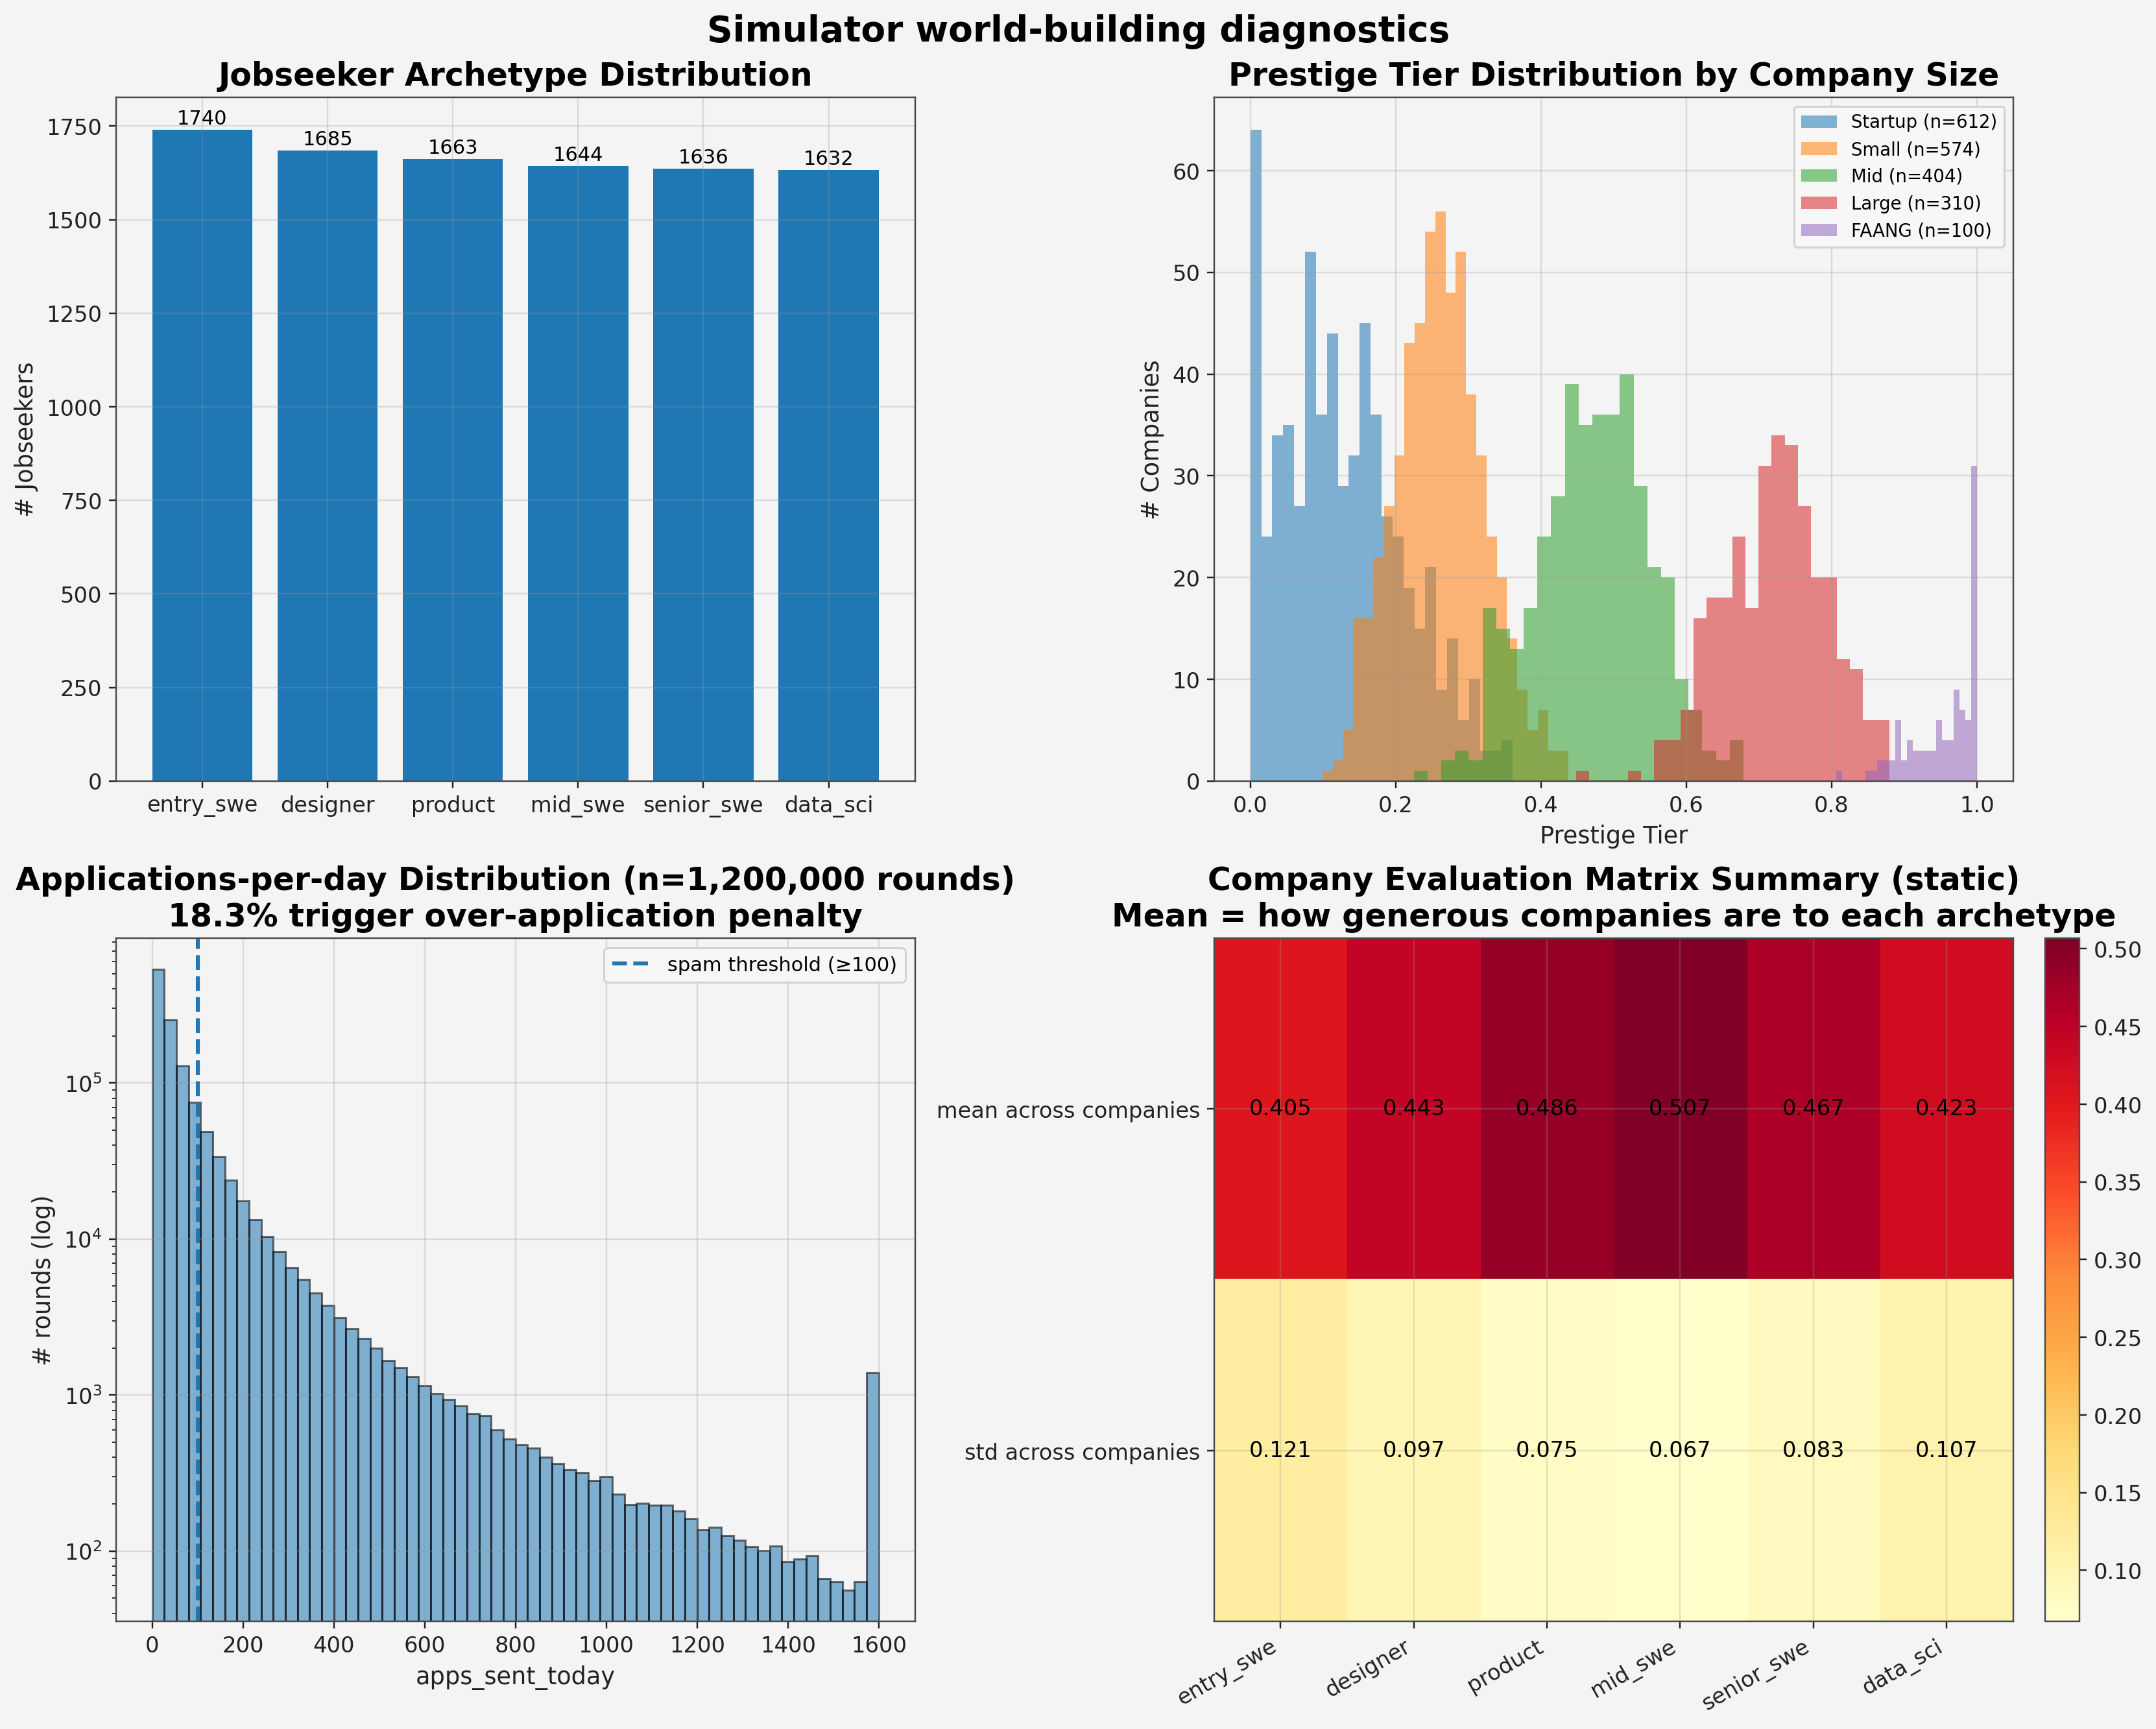
\includegraphics[width=\linewidth]{01_simulator_world_stats.png}
\caption{Simulator world statistics. (a)~Session-goal distribution;
(b)~company-tier distribution (heavy-tailed, few elite firms);
(c)~applicant-cohort distribution; (d)~outcome mix per algorithm --- the share
of \texttt{interview\_1}/\texttt{rejected}/\texttt{ignored} is similar across
algorithms ($\approx\!13\%$/$26\%$/$60\%$), so reward differences come from
many small per-round improvements rather than one dramatic jump.}
\label{fig:world}
\end{figure}

% ---------------------------------------------------------------------
\section{Methods}

\subsection{Problem formulation}

At round $t=1,\ldots,T$ the agent observes context $x_t\in\mathbb{R}^d$ with
$d=48$, selects an arm $a_t\in\mathcal{A}=\{\text{5 UI arms}\}$, and receives
scalar reward $r_t$ from \eqref{eq:reward}. Let
$\mu_t(a)=\mathbb{E}[r_t\mid x_t, a]$ be the oracle expected reward. The
context-dependent optimal arm is $a_t^\star=\arg\max_{a}\mu_t(a)$ and
\emph{expected contextual regret} is
\begin{equation}
R(T)\;=\;\sum_{t=1}^{T}\bigl[\mu_t(a_t^\star)-\mu_t(a_t)\bigr].
\label{eq:regret}
\end{equation}
This is our primary metric because it is lower-noise than realised regret and
isolates policy quality from stochastic outcome noise.

\subsection{Algorithms compared}

\textbf{Non-contextual baselines.}
Each baseline maintains per-arm statistics only; the context vector is ignored.
$\varepsilon$-Greedy picks the empirical-best arm with probability $1-\varepsilon$
and a uniform random arm otherwise ($\varepsilon=0.05$); UCB1 picks
$\arg\max_a \bar r_a + c\sqrt{\log t / n_a}$ with $c=\sqrt{2}$; Gaussian
Thompson Sampling samples from per-arm posteriors $\mathcal{N}(\bar
r_a,\sigma^2/n_a)$.

\textbf{LinUCB.}
Disjoint per-arm linear model with ridge regression (Li et al.\ 2010). Maintain
$A_a=I,\; b_a=\mathbf{0}$, compute $\hat\theta_a=A_a^{-1}b_a$, and pick
\begin{equation}
a_t\;=\;\arg\max_{a\in\mathcal{A}}\!\Bigl(x_t^{\!\top}\hat\theta_a
\;+\;\alpha\sqrt{x_t^{\!\top}A_a^{-1}x_t}\Bigr),
\label{eq:linucb}
\end{equation}
with $\alpha=0.5$. Update
$A_{a_t}\!\leftarrow\! A_{a_t}+x_tx_t^{\!\top},\;
b_{a_t}\!\leftarrow\! b_{a_t}+r_tx_t$. The bonus
$\alpha\sqrt{x_t^{\!\top}A_a^{-1}x_t}$ is a per-arm, per-context confidence
term that shrinks as the arm is pulled in similar contexts.

\textbf{Contextual Thompson Sampling.}
Bayesian linear bandit with Gaussian posteriors (Agrawal \& Goyal 2013).
Maintain $B_a,\,f_a$ with $\mu_a=B_a^{-1}f_a$, and at each round \emph{sample}
\begin{equation}
\tilde\theta_a \;\sim\; \mathcal{N}\!\bigl(\mu_a,\; v^{2}B_a^{-1}\bigr),
\qquad a_t = \arg\max_{a} x_t^{\!\top}\tilde\theta_a,
\label{eq:cts}
\end{equation}
with $v=0.35$. Updates are
$B_{a_t}\!\leftarrow\! B_{a_t}+x_tx_t^{\!\top},\;
f_{a_t}\!\leftarrow\! f_{a_t}+r_tx_t$. Sampling replaces the deterministic UCB
bonus with posterior sampling, which explores more aggressively early and
exploits more decisively as the posterior sharpens.

\subsection{Oracle and evaluation}

Because the world model is known, we compute $\mu_t(a)$ in closed form from the
generative reward equations for \emph{every} arm at every round during logging,
and record the oracle expected reward $\mu_t(a_t^\star)$ alongside each
interaction. All reported regret is expected (equation~\ref{eq:regret}), not
realised. The benchmark uses horizon $T=1{,}050{,}000$ per algorithm
($5{,}250{,}000$ algorithm-rounds total), single seed \texttt{4014}. At this
scale the Monte-Carlo noise on per-algorithm cumulative regret is negligible:
a within-trajectory bootstrap gives $95\%$ intervals of width $\approx\!\pm
0.3\%$ of the final value.

% ---------------------------------------------------------------------
\section{Experimental Analysis}
\label{sec:exp}

\subsection{The environment is genuinely contextual}

Figure~\ref{fig:landscape} shows the reward landscape: in each session-goal
context, one UI arm is clearly dominant, and \emph{which} arm dominates changes
sharply with the goal. \texttt{focused\_search} favours \texttt{panel\_split}
($89\%$ oracle-best share, \texttt{guided\_chat} second at $11\%$);
\texttt{broad\_exploration} favours \texttt{card\_grid} ($100\%$);
\texttt{panic\_apply} favours \texttt{swipe\_fast} ($87\%$); and
\texttt{casual\_browse} favours \texttt{hybrid\_ranked} ($93\%$). Mean oracle
reward also varies across goals ($0.192$ for \texttt{focused\_search} down to
$0.160$ for \texttt{panic\_apply}), so no globally-dominant arm exists. This is
the structural precondition under which contextual methods should outperform
non-contextual ones.

\begin{figure}[t]
\centering
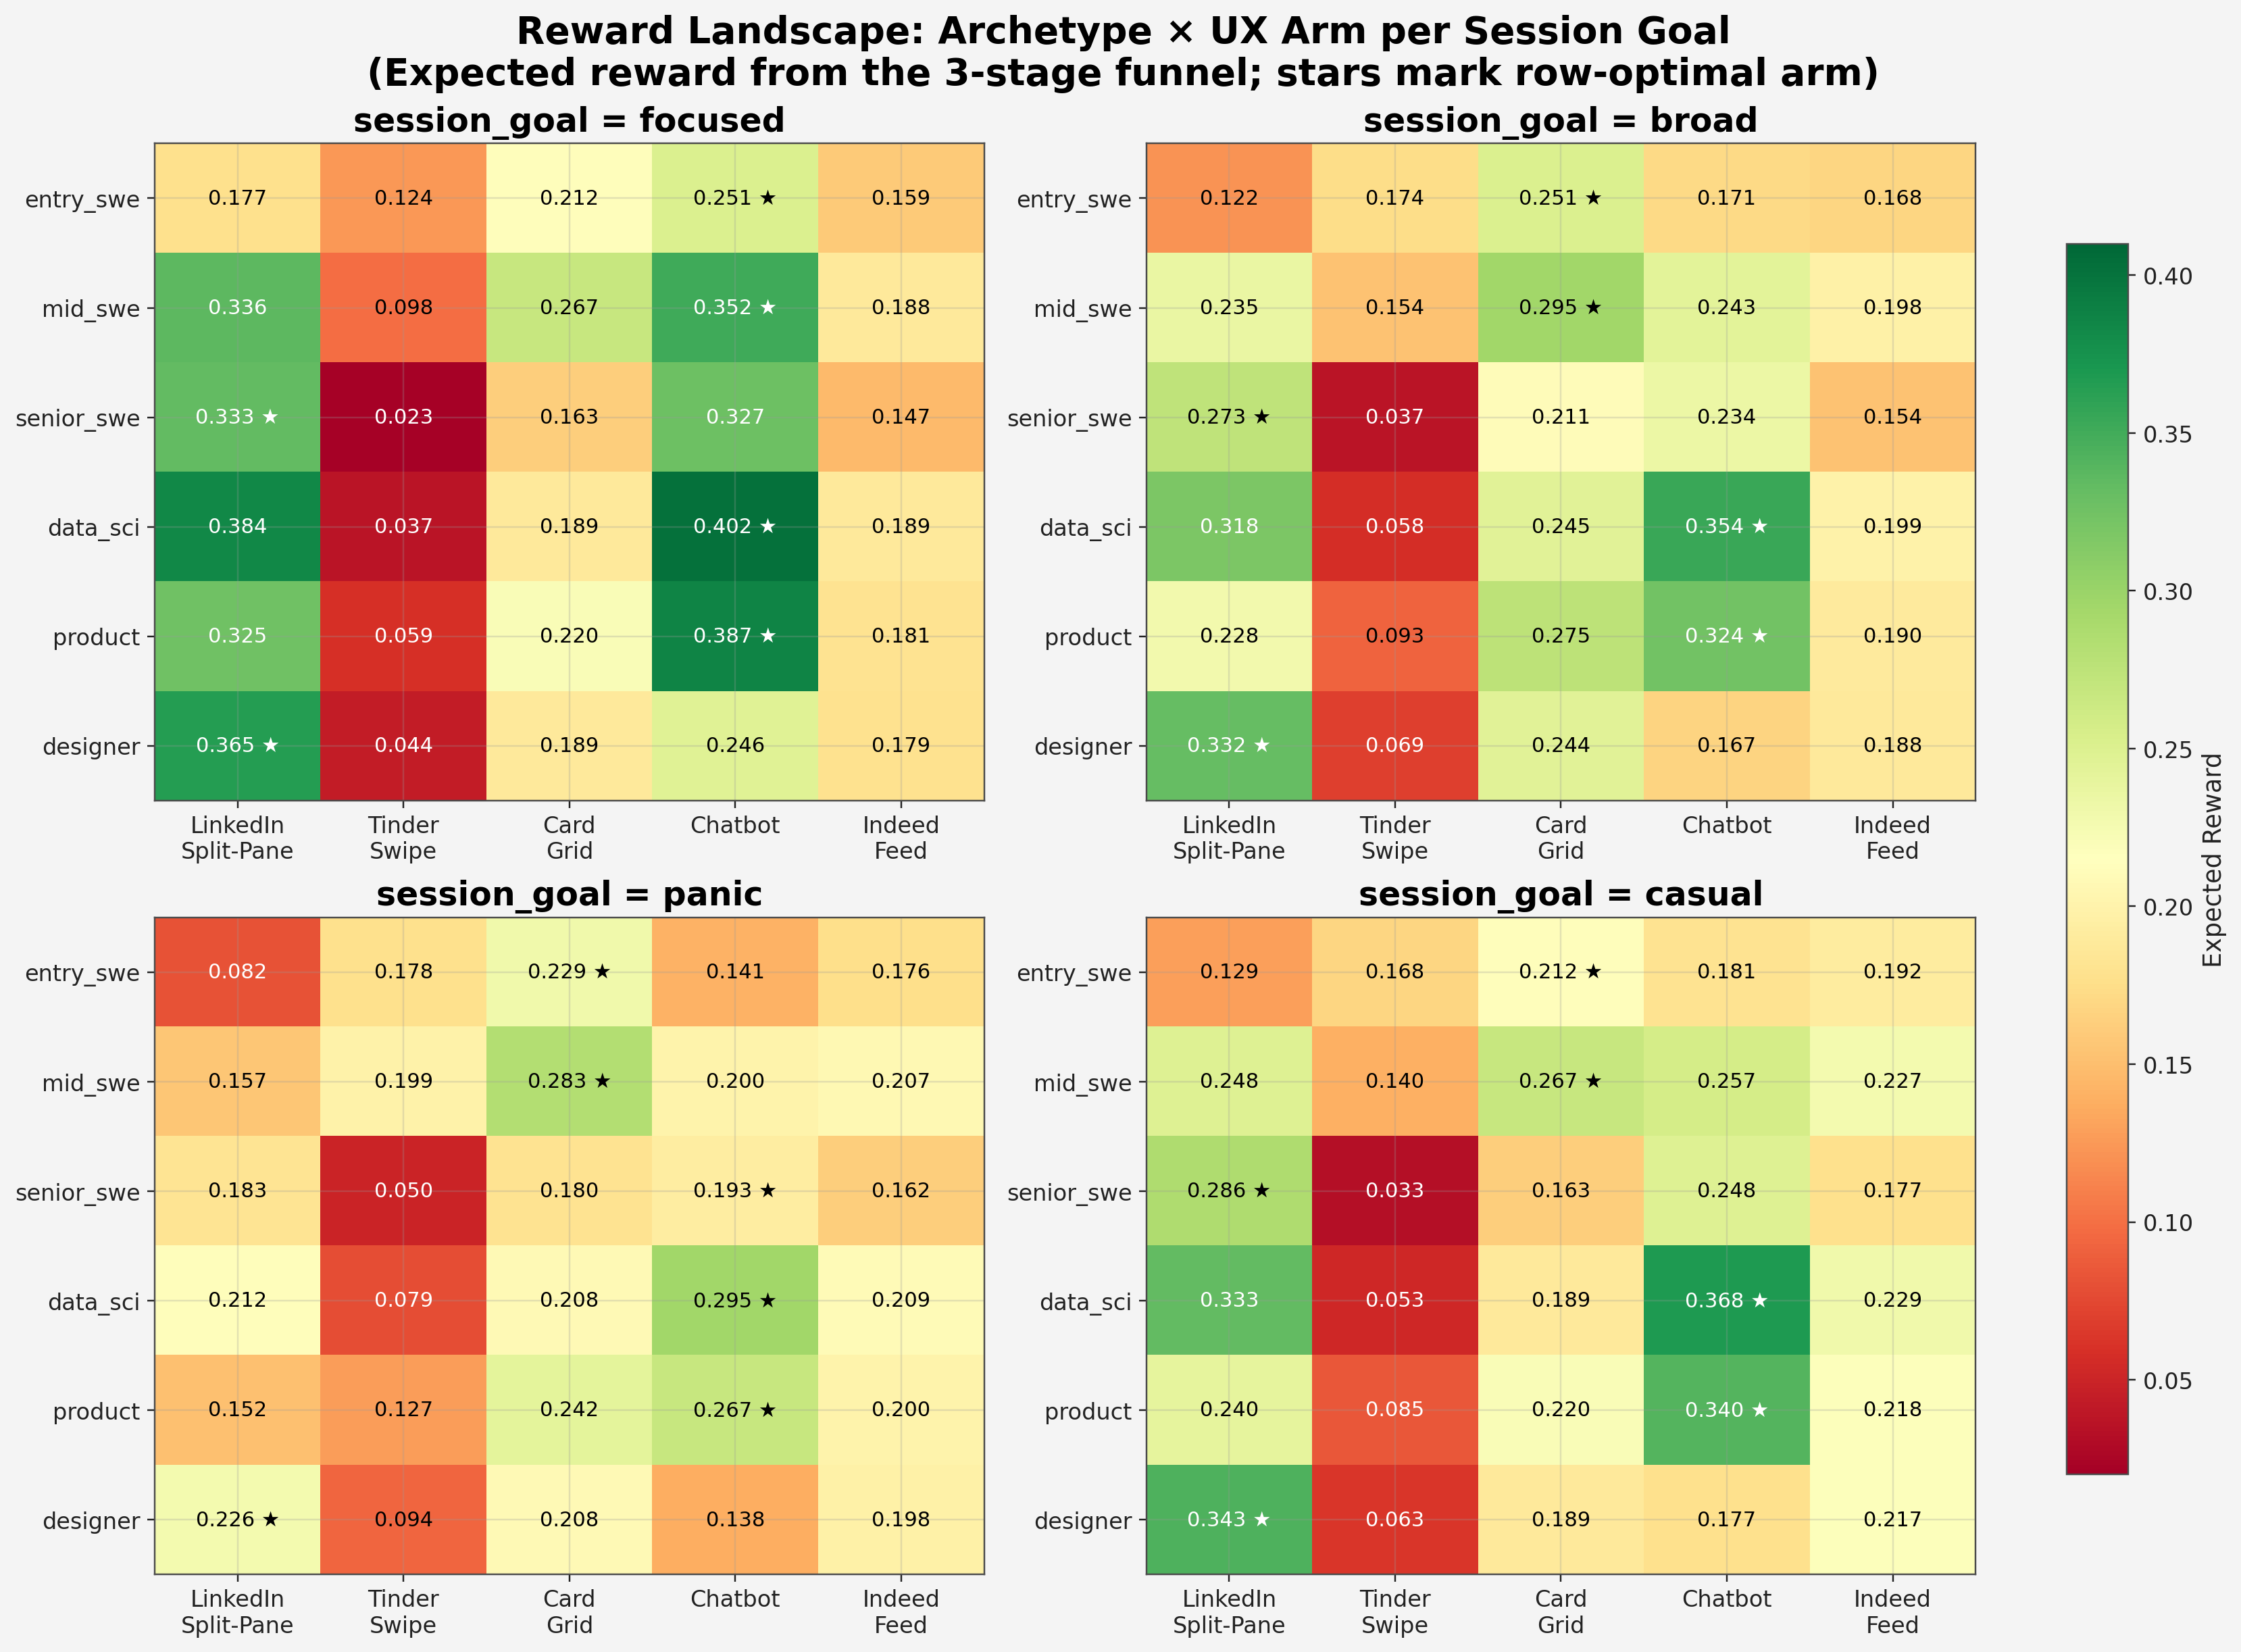
\includegraphics[width=0.96\linewidth]{02_reward_landscape_full.png}
\caption{Reward landscape by session goal. (a)~Fraction of rounds in each
context where a given UI arm is the oracle-best choice; the starred cell is
the row-best. (b)~Mean oracle expected reward when the arm \emph{is} the best
in that context. Different session goals have different preferred arms and
achievable reward levels, confirming the problem is truly contextual.}
\label{fig:landscape}
\end{figure}

\subsection{Main benchmark results}

Figure~\ref{fig:dashboard} reports the main online benchmark. Cumulative
expected regret (panel~a) separates the algorithms into two clear tiers:
Contextual TS and LinUCB trace nearly the same sublinear curve and finish at
$10{,}303$ and $11{,}029$ respectively, while $\varepsilon$-Greedy and Gaussian
TS accumulate almost twice as much regret ($19{,}447$ and $18{,}855$) and UCB1
finishes worst at $22{,}874$. Table~\ref{tab:policy-summary} lists final
numbers.

\begin{figure}[t]
\centering
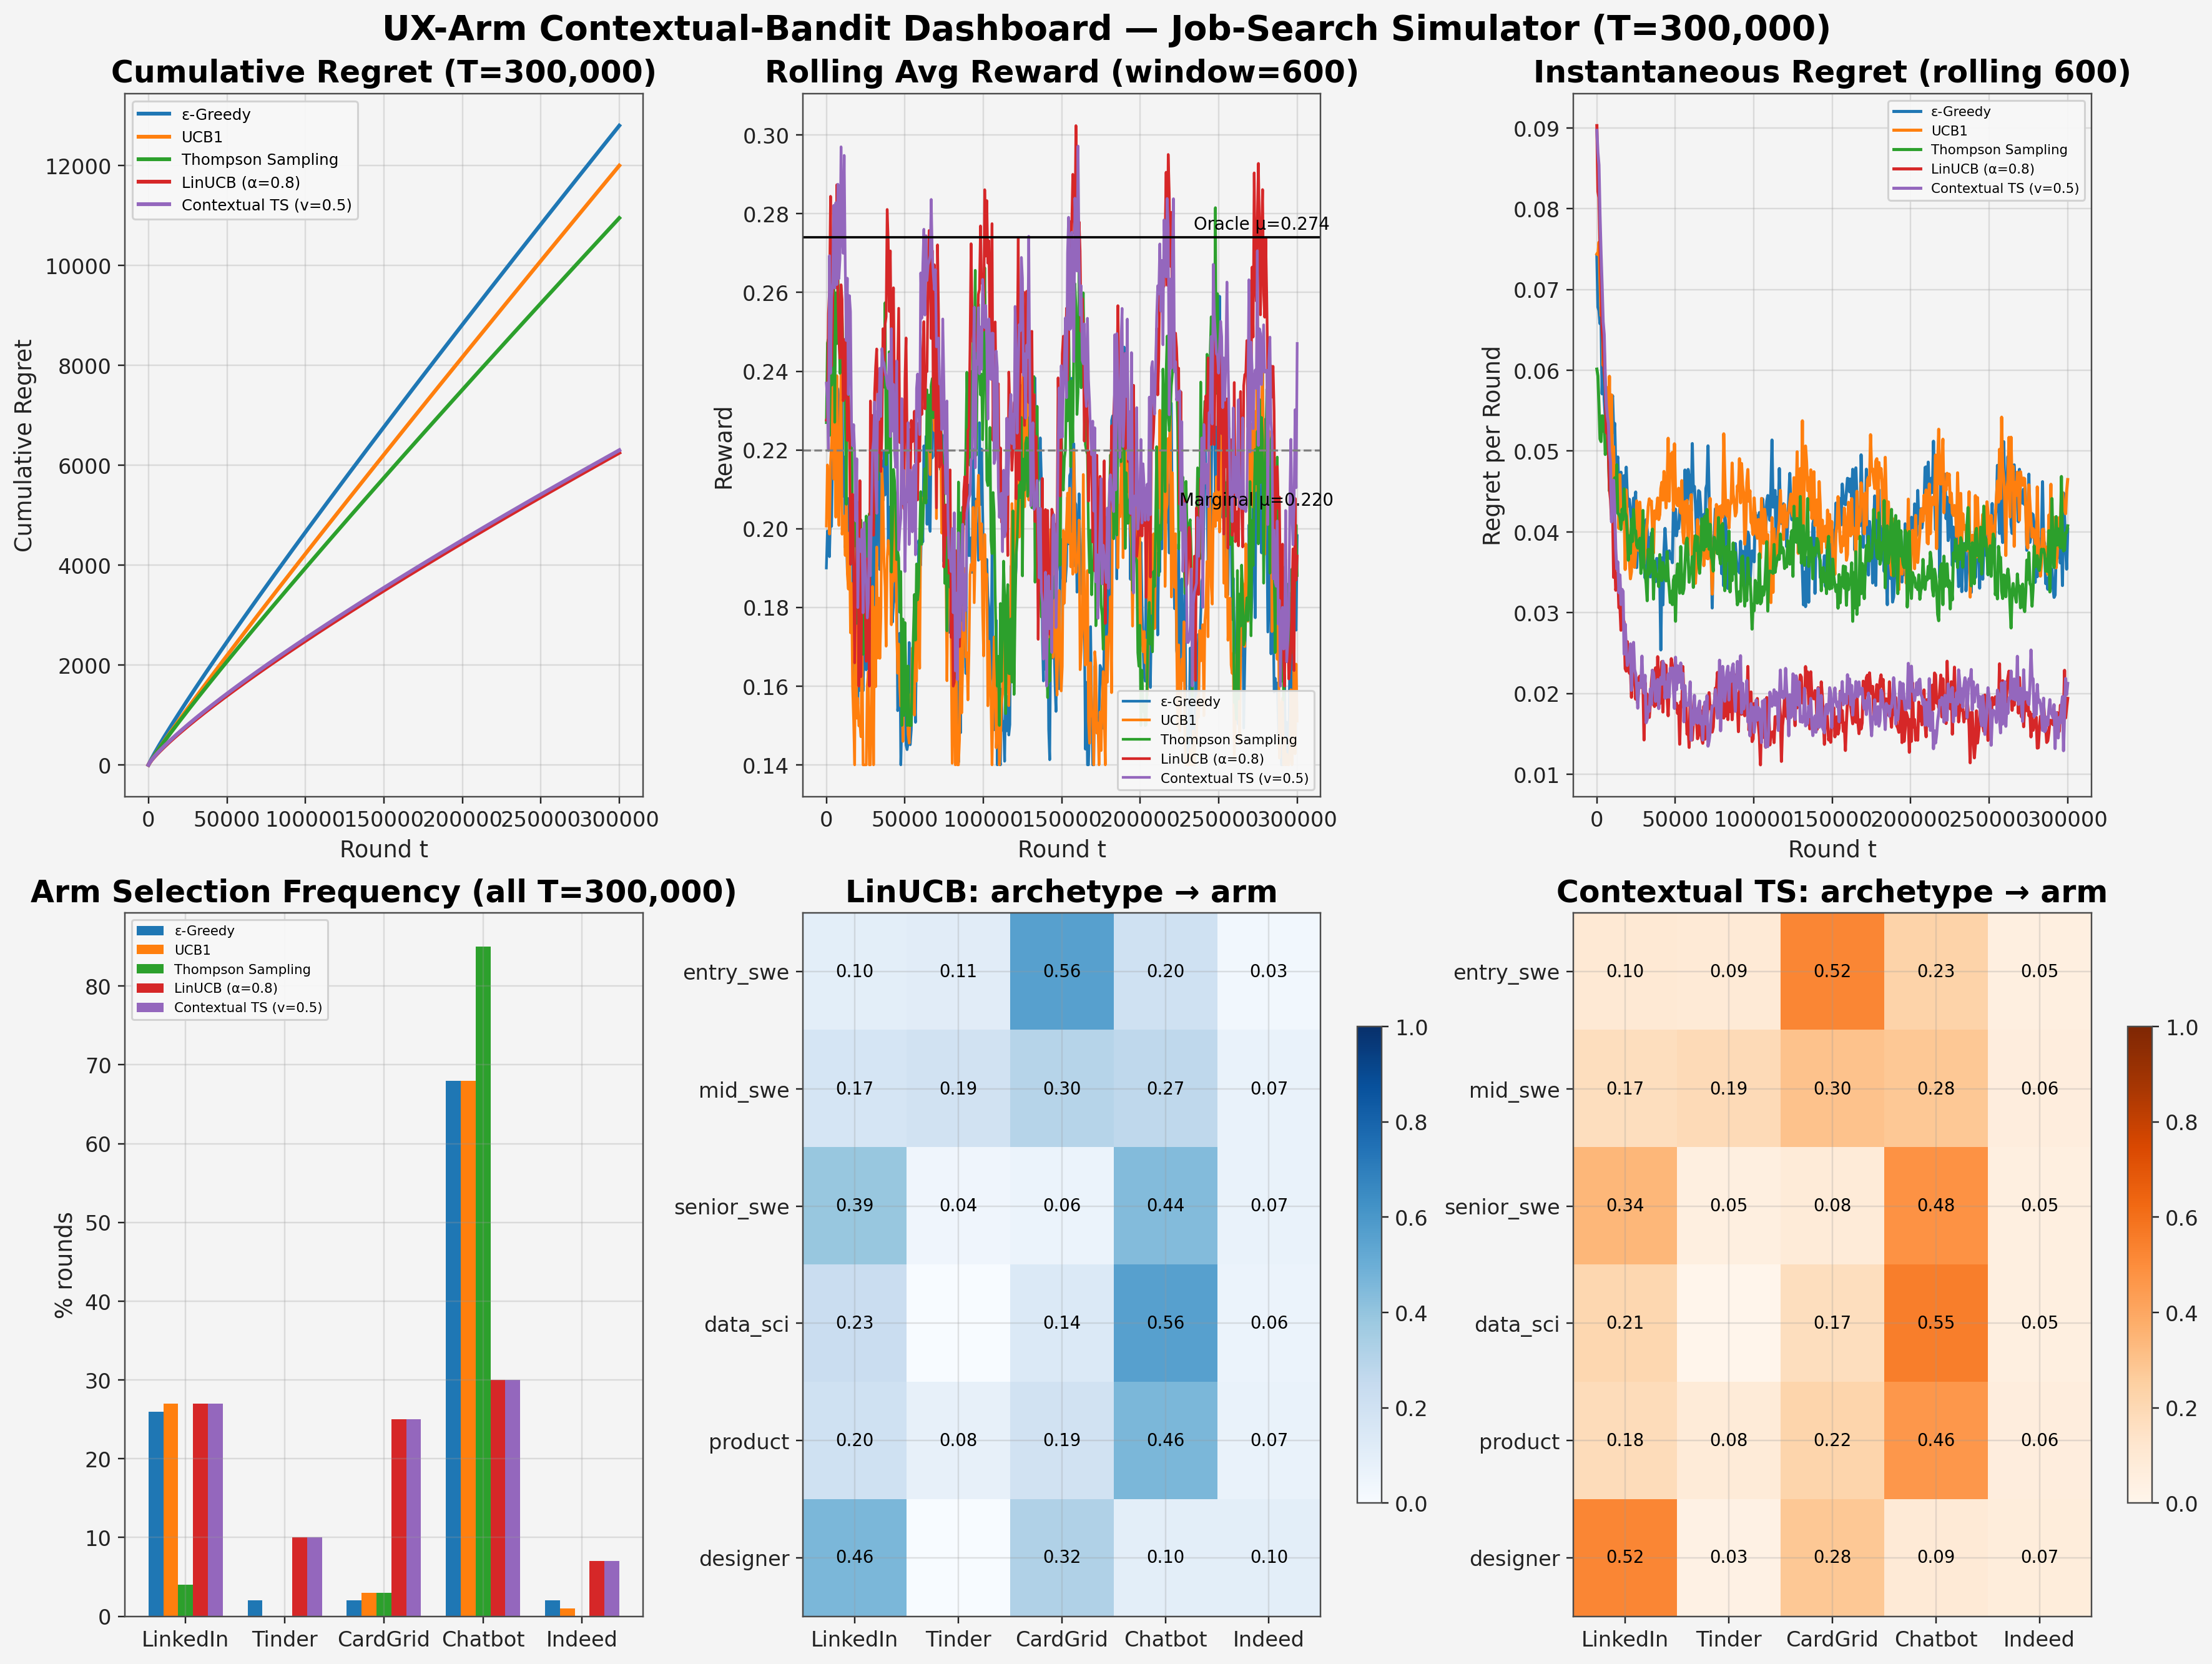
\includegraphics[width=\linewidth,height=0.40\textheight,keepaspectratio]{03_bandit_dashboard.png}
\caption{Main benchmark, $1{,}050{,}000$ rounds per algorithm. (a)~Cumulative
expected regret --- lower is better; contextual methods (red, orange) dominate
all non-contextual baselines and the gap widens over time. (b)~Final cumulative
regret. (c)~Rolling realised reward ($5{,}000$-round window); contextual
methods sit consistently above non-contextual ones. (d)~Arm selection
frequency: non-contextual methods collapse to $\sim\!80$--$87\%$
\texttt{panel\_split}, while contextual methods diversify across
\texttt{panel\_split}, \texttt{card\_grid}, and \texttt{hybrid\_ranked}.}
\label{fig:dashboard}
\end{figure}

\begin{table}[t]
\small
\centering
\begin{tabular}{lrrrrr}
\toprule
Policy              & Final $R(T)$ & $\Delta$ vs.\ $\varepsilon$-Greedy & Mean reward & Interview rate & Ignore rate \\
\midrule
\textbf{Contextual TS} & \textbf{10{,}302.83} & $-47.0\%$ & 0.1445 & 0.1385 & 0.5918 \\
\textbf{LinUCB}        & \textbf{11{,}028.82} & $-43.3\%$ & 0.1441 & 0.1382 & 0.5918 \\
Gaussian TS            & 18{,}854.90 & $-3.0\%$  & 0.1364 & 0.1337 & 0.6030 \\
$\varepsilon$-Greedy   & 19{,}447.20 & $0.0\%$   & 0.1372 & 0.1343 & 0.6047 \\
UCB1                   & 22{,}874.04 & $+17.6\%$ & 0.1341 & 0.1304 & 0.6136 \\
\bottomrule
\end{tabular}
\caption{Policy summary over the full $1.05$M-round online benchmark.
Contextual methods cut cumulative regret by $43$--$47\%$ versus the best
non-contextual baseline; the interview rate is also higher by $\approx\!0.4$
percentage points.}
\label{tab:policy-summary}
\end{table}

The non-contextual regret curves are almost linear, whereas Contextual TS and
LinUCB curve visibly sub-linearly, as expected for policies that successfully
learn per-context structure. Arm frequencies (panel~d) already suggest the
mechanism: $\varepsilon$-Greedy and Gaussian TS allocate most traffic to
\texttt{panel\_split} because it is the globally-best-on-average arm; the
contextual methods spread traffic across the three arms that are oracle-best
in \emph{some} context (\texttt{panel\_split}, \texttt{card\_grid},
\texttt{hybrid\_ranked}), in roughly equal thirds.

\subsection{Where contextual methods actually win --- and where they don't}

Aggregating regret across all rounds hides an important nuance.
Figure~\ref{fig:per-goal-advantage} breaks final regret down per session goal
(left) and expresses each non-baseline method as a percentage regret reduction
versus $\varepsilon$-Greedy (right). Contextual methods win big in
\texttt{focused\_search} ($+44$ to $+49\%$), \texttt{broad\_exploration}
($+59$ to $+60\%$), and \texttt{casual\_browse} ($+80$ to $+81\%$), but
\emph{lose} in \texttt{panic\_apply} ($-7\%$ for Contextual TS, $-26\%$ for
LinUCB). This is an honest finding and a useful design lesson: in
\texttt{panic\_apply} the oracle arm (\texttt{swipe\_fast}) is so dominant that
the exploration budget of a contextual bandit is wasted, whereas
$\varepsilon$-Greedy's near-greedy behaviour works well. A production system
should detect obviously panic-apply sessions and hard-code \texttt{swipe\_fast}
for them rather than let a general contextual bandit explore.

\begin{figure}[t]
\centering
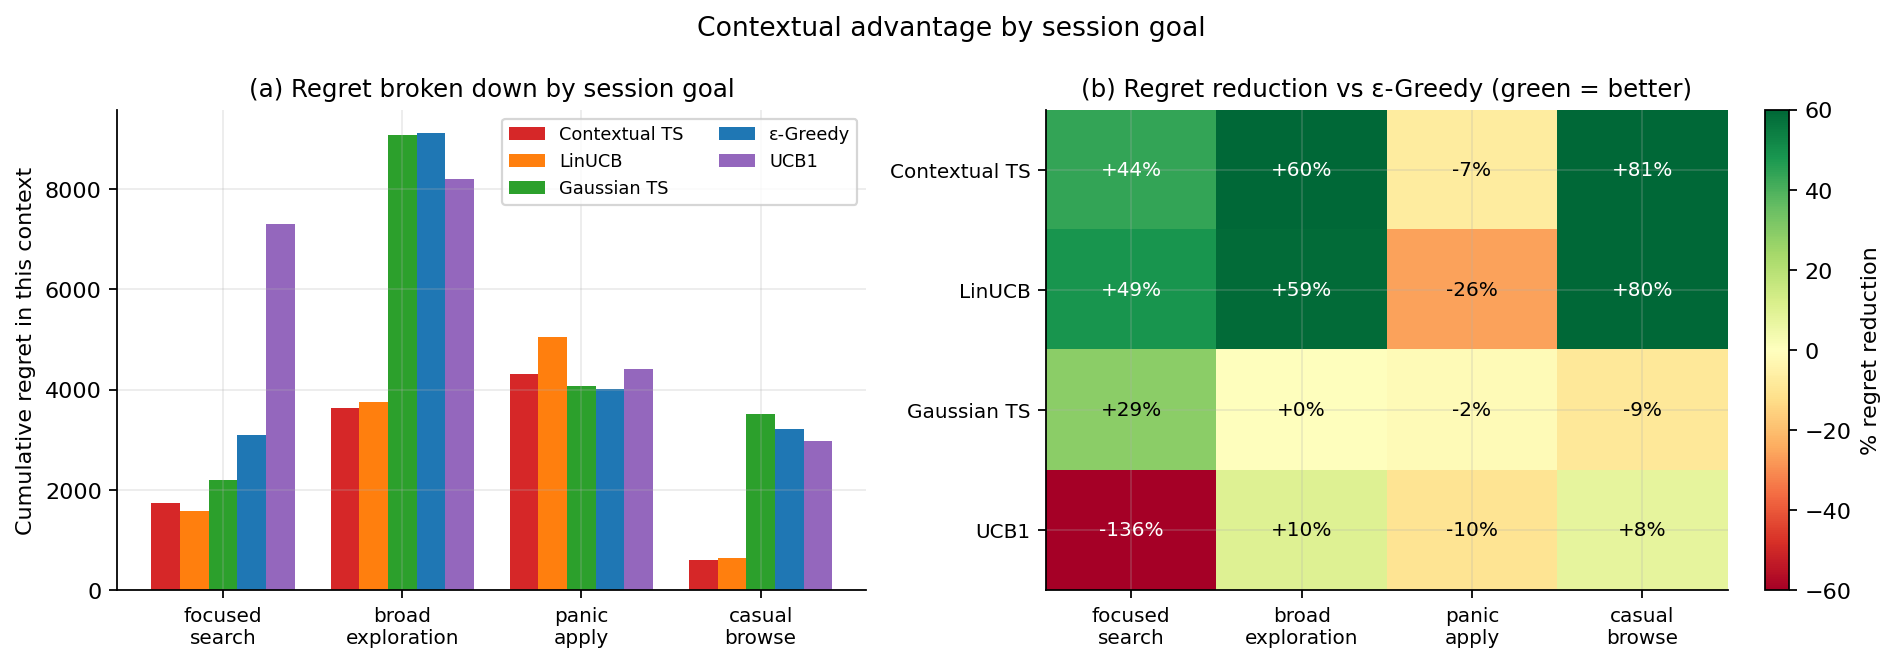
\includegraphics[width=\linewidth]{04_offline_bootstrap_replay.png}
\caption{Contextual advantage by session goal. (a)~Per-session-goal cumulative
regret. (b)~Percentage regret reduction versus $\varepsilon$-Greedy; green is
better than baseline, orange/red is worse. The advantage is large and
consistent except in \texttt{panic\_apply}, where exploration hurts.}
\label{fig:per-goal-advantage}
\end{figure}

\subsection{Learned policies --- contextual vs.\ collapse}

Figure~\ref{fig:learned-policy} is the single clearest view of the mechanism.
For each algorithm we plot the fraction of rounds it picks each arm within
each session-goal context. Contextual TS and LinUCB route arms per context
--- favouring \texttt{panel\_split} for \texttt{focused\_search}
($85$--$87\%$), \texttt{card\_grid} for \texttt{broad\_exploration}
($58$--$62\%$), and \texttt{hybrid\_ranked} for \texttt{casual\_browse}
($69$--$85\%$) --- which closely follows the oracle landscape in
Figure~\ref{fig:landscape}. Non-contextual methods collapse: Gaussian TS and
$\varepsilon$-Greedy pick \texttt{panel\_split} for $\sim\!81$--$87\%$ of
\emph{every} context. UCB1 is still spreading traffic nearly uniformly --- its
exploration term has not shrunk enough at $T=1.05$M for a clean policy to
emerge. The contextual policies recover a coarse version of the oracle
landscape from data alone, without any supervision; the non-contextual
policies structurally \emph{cannot} represent that mapping and are forced to
serve one arm everywhere.

\begin{figure}[t]
\centering
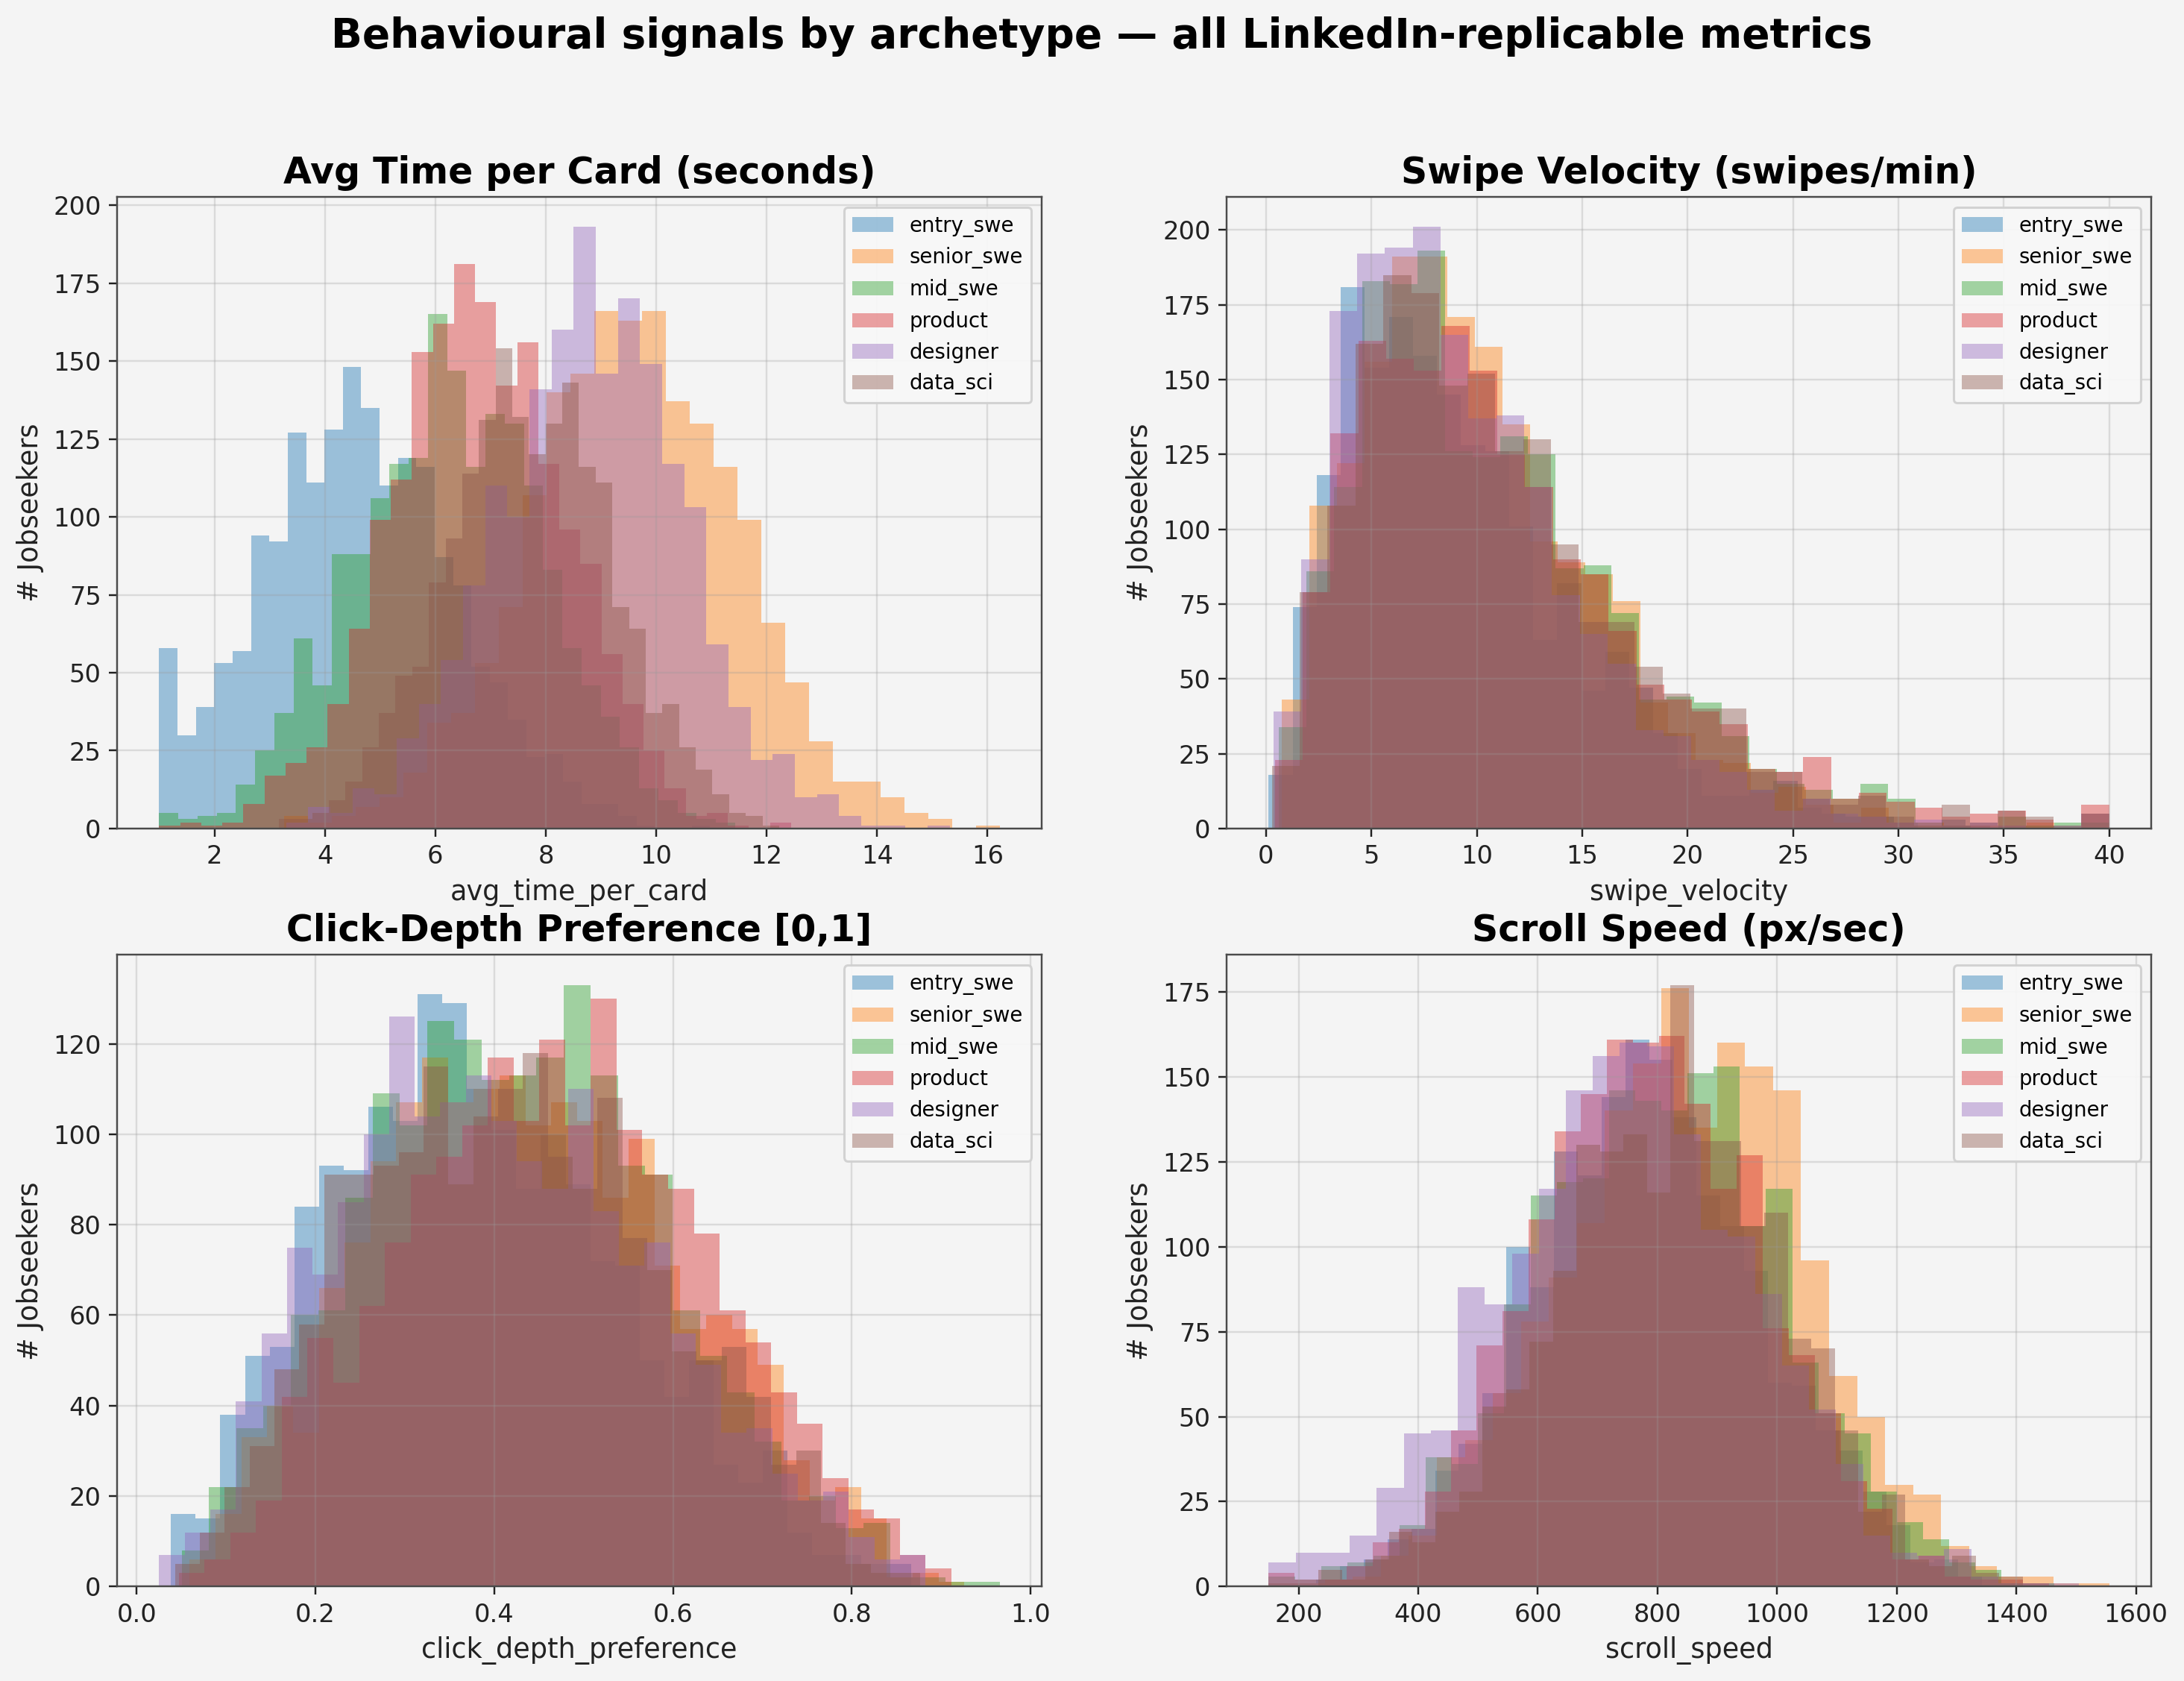
\includegraphics[width=\linewidth]{05_behavioural_signals.png}
\caption{Learned policy per (algorithm~$\times$~session goal), as a share
(\%) of rounds. Contextual methods (two leftmost panels) route arms by
context; non-contextual methods (three rightmost) do not.}
\label{fig:learned-policy}
\end{figure}

% ---------------------------------------------------------------------
\section{Conclusions}

We built a $48$-dimensional contextual-bandit environment for adaptive
job-search UI selection with five competing UI arms and four session-goal
contexts that induce a non-trivial reward landscape. Evaluated across $1.05$M
interaction rounds per policy, context-aware methods (Contextual TS, LinUCB)
cut cumulative expected regret by $43$--$47\%$ versus the best non-contextual
baseline and recover a coarse version of the oracle policy from data.
Contextual methods route arms by session goal, while non-contextual methods
collapse to whichever arm has the highest global mean
(\texttt{panel\_split}). The result is not uniform across contexts, which we
treat as a feature rather than a bug: in \texttt{panic\_apply} the oracle arm
is so dominant that exploration hurts. A production system should combine a
lightweight heuristic on obvious session signals with a contextual bandit on
the remaining traffic.

\textbf{Limitations.}
All results are from a single seed of a synthetic world with a known reward
model; real platforms have non-stationary populations and unobserved
confounders we do not model. LinUCB and Contextual TS use linear reward models
--- a valid first step, but a production deployment would likely extend this
with nonlinear features or deep contextual bandits. Our oracle baseline uses
privileged access to the simulator's expected-reward function; a real-world
deployment would have to estimate a value function from logged interactions.
Finally, we treat the company evaluation rubric as static; a full system must
also cope with evaluator drift.

\textbf{Code and data.}
All code, the notebook that regenerates every figure in this report, and the
$5.25$M-row experiment parquet are available at\\
\url{https://github.com/codegrox/job-ui-contextual-bandits} (large artefacts
via Git LFS).

% ---------------------------------------------------------------------
\newpage
\section*{AI Use Acknowledgment}
\small

We used AI tools like Google Gemini, GPT 5.5 and Claude Opus 4.6 to support parts of the workflow, including notebook cleanup, figure narration, LaTeX/report polishing, repository organization, and wording refinement. All simulator design decisions, experiment execution, figure selection, and final interpretation remained the responsibility of the group.

\vspace{0.6em}
\footnotesize\noindent\textbf{References.}
Li, Chu, Langford \& Schapire (2010), \emph{A contextual-bandit approach to
personalized news article recommendation}, WWW'10. \;
Agrawal \& Goyal (2013), \emph{Thompson sampling for contextual bandits with
linear payoffs}, ICML'13. \;
Auer, Cesa-Bianchi \& Fischer (2002), \emph{Finite-time analysis of the
multiarmed bandit problem}, Machine Learning 47.

\end{document}
